\documentclass[12pt]{article}
\usepackage{amsmath}
\usepackage{graphicx}
\usepackage{enumerate}
\usepackage{natbib}
\usepackage{url}
\usepackage{enumitem}
\usepackage[dvipsnames]{xcolor}

\usepackage{amsmath,amssymb,amsthm,bm,mathtools}
\usepackage{algorithm}
\usepackage{dsfont,multirow,hyperref,setspace,enumerate}
\hypersetup{colorlinks,linkcolor={black},citecolor={black},urlcolor={black}}


\newcommand{\blind}{1}


% DON'T change margins - should be 1 inch all around.
\addtolength{\oddsidemargin}{-.5in}%
\addtolength{\evensidemargin}{-.5in}%
\addtolength{\textwidth}{1in}%
\addtolength{\textheight}{1.3in}%
\addtolength{\topmargin}{-.8in}%


\theoremstyle{definition}
\newtheorem{thm}{Theorem}[section]
\newtheorem{lem}{Lemma}[section]
\newtheorem{prop}{Proposition}[section]
\newtheorem{pro}{Property}[section]
\newtheorem{cor}{Corollary}[section]

\newtheorem{assumption}{Assumption}[section]
\newtheorem{defn}{Definition}[section]
\newtheorem{example}{Example}[section]
\newtheorem{rmk}{Remark}[section]


\newtheorem{innercustomgeneric}{\customgenericname}
\providecommand{\customgenericname}{}
\newcommand{\newcustomtheorem}[2]{%
  \newenvironment{#1}[1]
  {%
   \renewcommand\customgenericname{#2}%
   \renewcommand\theinnercustomgeneric{##1}%
   \innercustomgeneric
  }
  {\endinnercustomgeneric}
}

\newcustomtheorem{customexample}{Example}

\usepackage{appendix}
\usepackage{wrapfig}
\mathtoolsset{showonlyrefs}

%This is for cross reference in overleaf
\usepackage{xr}
\makeatletter
\newcommand*{\addFileDependency}[1]{% argument=file name and extension
  \typeout{(#1)}
  \@addtofilelist{#1}
  \IfFileExists{#1}{}{\typeout{No file #1.}}
}
\makeatother

\newcommand*{\myexternaldocument}[1]{%
    \externaldocument{#1}%
    \addFileDependency{#1.tex}%
    \addFileDependency{#1.aux}%
}
\myexternaldocument{jcgs-tensor}



\input macros.tex


\usepackage[english]{babel}

\newcommand*{\KeepStyleUnderBrace}[1]{%f
  \mathop{%
    \mathchoice
    {\underbrace{\displaystyle#1}}%
    {\underbrace{\textstyle#1}}%
    {\underbrace{\scriptstyle#1}}%
    {\underbrace{\scriptscriptstyle#1}}%
  }\limits
}


\usepackage{algpseudocode,algorithm}
\algnewcommand\algorithmicinput{\textbf{Input:}}
\algnewcommand\algorithmicoutput{\textbf{Output:}}
\algnewcommand\INPUT{\item[\algorithmicinput]}
\algnewcommand\OUTPUT{\item[\algorithmicoutput]}

\def\ci{\perp\!\!\!\perp}

\def\fixme#1#2{\textbf{\color{red}[FIXME (#1): #2]}}
\usepackage{booktabs}
\newcommand\doubleRule{\toprule\toprule}
\allowdisplaybreaks


\usepackage[compact]{titlesec}


\begin{document}



\def\spacingset#1{\renewcommand{\baselinestretch}%
{#1}\small\normalsize} \spacingset{1.5}




%%%%%%%%%%%%%%%%%%%%%%%%%%%%%%%%%%%%%%%%%%%%%%%%%%%%%%%%%%%%%%%%%%%%%%%%%%%%%%
\begin{center}
{\Large\bf Supplementary Notes to ``Supervised tensor decomposition with features on multiple modes''}

\vspace{.5cm}

{\large Jiaxin Hu, Chanwoo Lee, Miaoyan Wang}\\
University of Wisconsin-Madison

\vspace{.5cm}
\end{center}
\appendix
\renewcommand{\thefigure}{S\arabic{figure}}
\setcounter{figure}{0}   
\renewcommand{\thetable}{S\arabic{table}}
\setcounter{table}{0}   



The supplementary note consists of proofs (Section~\ref{sec:appendix}), additional simulation results (Section~\ref{sec:asimulation}), and data applications (Section~\ref{sec:adata}).

\section{Proofs}\label{sec:appendix}
\subsection{Proof of Theorem~\ref{thm:MLE}}
We denote several quantities:
\begin{equation}\label{eq:quantities}
\underline \gamma = \prod_{k\in[K]} \sigma_{\min}(\mX_k),\quad \bar \gamma =\prod_{k\in[K]}\sigma_{\max}(\mX_k),  \quad \lambda =\min_{k\in[K]}\sigma_{\min}(\text{Unfold}_k(\tB_{\text{true}})),
\end{equation}
where $\underline{\gamma}$ quantifies the rank non-deficiency of feature matrices, $\bar \gamma$ quantifies the magnitude of feature matrices, and $\lambda$ is the smallest singular value of mode-$k$ unfolded matrices $\text{Unfold}_k(\trueB)$ for all possible $k\in[K]$. 
For notational convenience, we drop the subscript $\tY$ from the objective $\tL_\tY(\cdot)$ and simply write as $\tL(\cdot)$. We write $\tL(\tB)$ in place of $\tL(\tC, \mM_1,\ldots,\mM_K)$ when we want to emphasize the role of $\tB$. 

\begin{prop}[sub-Gaussian residuals]\label{prop}
Define the residual tensor $\tE=\entry{\varepsilon_{i_1,\ldots,i_K}}=\tY-b'(\Theta)\in\mathbb{R}^{d_1\times \cdots \times d_K}$. Under the Assumption A2, $\varepsilon_{i_1,\ldots,i_K}$ is a sub-Gaussian random variable with sub-Gaussian parameter bounded by $\phi U$, for all $(i_1,\ldots,i_K)\in[d_1]\times\cdots\times[d_K]$.
\end{prop}

\begin{prop}[Properties of tensor GLM]\label{lem}Consider tensor GLMs under Assumption A2.
\begin{enumerate}[label=(\alph*)]
\item (Strong convexity) For all $\tB$ and all realized data tensor $\tY$,
\[
\tL(\trueB)\geq \tL(\tB)+ \langle \nabla \tL(\tB_{\text{true}}), \trueB-\tB \rangle+{1\over 2} \underline{\gamma}^2L\FnormSize{}{\trueB-\tB}^2,
\] 
where $\nabla L(\cdot)$ denotes the derivative of $\tL$ with respect to $\tB$.   
\item (Model complexity) 
Suppose $\tY$ follows generalized tensor model with parameter $\trueB$. Then, with probability at least $1-\exp(-p)$, 
\begin{equation}\label{eq:b}
\text{Err}_{\text{ideal}}(\mr):= \sup_{\substack{ \FnormSize{}{\tB}=1, \tB\in\tP(\mr)}}\langle \nabla \tL(\tB_{\text{true}}), \tB \rangle\lesssim \bar \gamma \sqrt{\phi U(r^K+Kpr)}. 
\end{equation}
\end{enumerate}
\end{prop}
The proofs of Propositions~\ref{prop}-\ref{lem} are in Section~\ref{sec:lemma}. 

\begin{proof}[Proof of Theorem~\ref{thm:MLE}]
First we prove the error bound for $\MLEB$. By the definition of $\MLEB$, $\tL_{\tY}(\trueB)-\tL_{\tY}(\MLEB)\leq 0$. By the strong convexity in Proposition~\ref{lem},
\begin{align}\label{eq:F-norm}
0&\geq \tL_{\tY}(\trueB)- \tL_{\tY}(\MLEB)  \geq \langle \nabla \tL(\tB_{\text{true}}), \trueB-\MLEB \rangle+{1\over 2}\underline{\gamma}^2L\FnormSize{}{\trueB-\MLEB}^2.
\end{align}
Rearranging~\eqref{eq:F-norm} gives
\[
\FnormSize{}{\MLEB-\trueB}\leq {2\over \underline{\gamma}^2L} \left\langle \nabla \tL(\tB_{\text{true}}), {\MLEB-\trueB\over\FnormSize{}{\MLEB-\trueB}} \right\rangle\leq {2\over \underline{\gamma}^2L}  \text{Err}_{\text{ideal}}(2\mr),
\]
where the last inequality comes from the definition of $\text{Err}_{\text{ideal}}(2\mr)$ and the fact that $\text{rank}(\MLEB-\trueB)\leq \text{rank}(\MLEB)+\text{rank}(\trueB)\leq 2\mr$. By~\eqref{eq:b} in Proposition~\ref{lem}, we have 
\begin{equation}\label{eq:Bbound}
\FnormSize{}{\MLEB-\trueB} \lesssim {\bar \gamma \sqrt{\phi U}\over \underline{\gamma}^2 L}\sqrt{r^K+Kpr},
\end{equation}
with probability at least $1-\exp(-p)$.

Now, we specialize $\bar \gamma/\underline{\gamma}^2 $ in the following two cases of assumptions on feature matrices. 
\begin{itemize}[leftmargin=0cm]
\item[] [Case 1] Under Assumption A1 with scaled feature matrices, we have
\begin{equation}\label{eq:case1}
{\bar \gamma\over \underline{\gamma}^2} \leq {c^K_2d^{K/2} \over c^{2K}_1d^{K}} \lesssim \sqrt{1\over d^{K}}.
\end{equation}
\item[] [Case 2] Under Assumption A1' with original feature matrices, the asymptotic behavior of extreme singular values \citep{rudelson2010non} are
\[
\sigma_{\min}(\mX_k) \asymp \sqrt{d}-\sqrt{p} \text{ and  } \sigma_{\max}(\mX_k) \asymp \sqrt{d}+\sqrt{p},\quad \text{for all }k\in[K].
\]
In this case, we obtain 
\begin{equation}\label{eq:case2}
{\bar \gamma\over \underline{\gamma}^2} \asymp {(\sqrt{d}+\sqrt{p})^{K} \over (\sqrt{d}-\sqrt{p})^{2K}} \lesssim \sqrt{1\over d^K}.
\end{equation}
\end{itemize}
Combining~\eqref{eq:Bbound} with either~\eqref{eq:case1} or~\eqref{eq:case2}, in both cases we obtain the same conclusion
\begin{equation}\label{eq:bound2}
\FnormSize{}{\MLEB-\trueB}^2\lesssim {\phi(r^K+Kpr)\over d^K}.
\end{equation}
Now we prove the bound for sin$\Theta$ distance. 
We unfold tensors $\trueB$ and $\MLEB$ along the mode $k$ and obtain $\text{Unfold}_k(\trueB)$ and $\text{Unfold}_k(\MLEB)$. Notice that $\trueM$ and $\hat \mM_{k,\textup{MLE}}$ span the top-$r$ left singular spaces of $\text{Unfold}_k(\trueB)$ and $\text{Unfold}_k(\MLEB)$, respectively.  Applying Proposition~\ref{prop:sinebound} to this setting gives
\begin{align}\label{eq:sintheta}
    \text{sin}\Theta(\trueM,\hat\mM_{k,\textup{MLE}})\leq \frac{\FnormSize{}{\text{Unfold}_k(\MLEB)-\text{Unfold}_k(\trueB)}}{\sigma_{\text{min}}(\text{Unfold}_k(\trueB))}= \frac{\FnormSize{}{\MLEB-\trueB}}{\lambda}.
    \end{align}
The proof is complete by combining~\eqref{eq:bound2} and~\eqref{eq:sintheta}.
\end{proof}


\subsection{Proofs of Proposition~\ref{lem:ini} and Theorem~\ref{thm:local}}
\begin{proof}[Proof of Proposition~\ref{lem:ini}]

We express the Gaussian model as 
\begin{align}\label{eq:gaussian}
    \tY = \tB_{\text{true}}\times \{\mX_1,\ldots,\mX_K\} + \tE,
\end{align}
where $\tE$ is a noise tensor consisting of i.i.d.\ entries from $N(0,\sqrt{\phi}).$ 
By QR decomposition on feature matrices, $\mX_k = \mQ_k\mR_k$ for all $k\in[K]$, we have 
\begin{align}\label{eq:gaussian2}
    \bar\tY = \tB_{\text{true}}\times\{\mR_1,\ldots \mR_K\}+\bar\tE,
\end{align}
where $\bar\tY = \tY\times\{\mQ_1,\ldots,\mQ_K\}$ and  $\bar\tE = \tE\times\{\mQ_1,\ldots,\mQ_K\}$.
Notice that entries of $\bar\tE\in\mathbb{R}^{p\times\cdots\times p}$ are i.i.d drawn from $N(0,\sqrt{\phi})$ by the orthonormality of $\{\mQ_k\}_{k=1}^K$. Reparameterize the signal in \eqref{eq:gaussian2} as 
\begin{align}\label{eq:repara}
    \tS_{\text{true}} := \tB_{\text{true}}\times\{\mR_1,\ldots \mR_K\}&=  \tC_{\text{true}}\times\{\mR_1\mM_{1,\text{true}},\ldots \mR_K\mM_{K,\text{true}}\}\notag \\
    & = \tC'_{\text{true}}\times\{\mU_{1,\text{true}},
    \ldots,\mU_{K,\text{true}}\},
\end{align}
where $\mU_{k.\text{true}}\in\mathbb{O}(p_k, r_k)$ are orthonormal matrices and $\tC'_{\text{true}}\in\mathbb{R}^{r\times \cdots\times r}$ is a full rank core tensor.
By definition of quantities in \eqref{eq:quantities}, we have
\begin{align}\label{eq:lambdas}
    \lambda' := \min_{k\in[K]}\sigma_{\min}(\text{Unfold}_k(\tS_{\text{true}}))\in[  \lambda \underline \gamma,\ \lambda \bar \gamma].
\end{align}

Now our setup shares the same setting as in~\citet[Theorem 1]{zhang2018tensor}.
We summarize the relationships between our algorithm outputs and the ones in \cite{zhang2018tensor}. For all $k\in[K],$
\begin{enumerate}
    \item  $\mM_{k,\text{true}} = \text{SVD}_{r_k}\left(\mR_k^{-1}\mU_{k,\text{true}}\right):=$  the first $r_k$ left singular vectors of $\mR_k^{-1}\mU_{k,\text{true}}$;
   % \item $\hat\mM^{(0)}_k = \hat \mU_k^{(0)}$.
    \item $\hat\mM_{k}^{(t)} = \text{SVD}_{r_k}\left(\mR_k^{-1}\hat\mU_{k}^{(t)}\right)$ for all $t=0,1,2,\ldots$;
\end{enumerate}
where $\hat \mU^{(t)}_k$ denotes the $t$-th iteration output of Higher Order Orthogonal Iteration (HOOI) algorithm \citep{zhang2018tensor} with inputs $\bar \tY$. 
The first relationship is from~\eqref{eq:repara}, and second relationship is from induction by $t$. Briefly, $t=0$ holds because of the definition  $\hat\mM^{(0)}_k$ based on lines 4-5 of our initialization Algorithm~\ref{alg:A}. For $t\geq 1,\ldots$, notice that $\hat\mM_k^{(t)}$ is an optimizer of the objective \[\FnormSize{}{\bar\tY-\hat\tC^{(t-1)}\times\{\mR_1\hat\mM_1^{(t)},\ldots,\mR_{k-1}\hat\mM_{k-1}^{(t)},\mR_k\mM,\mR_{k+1}\hat\mM_{k+1}^{(t-1)},\ldots,\mR_K\hat\mM^{(t-1)}_K\}}^2,\]
from the line 3 of  Algorithm~\ref{alg:B}. By unfolding along the mode $k$, the optimizer $\mM_k^{(t)}$ must satisfy
\begin{align}\label{eq:HOOI}
    \text{Unfold}_k&\left(\bar\tY\times\left\{ (\hat\mM_1^{(t)})^T\mR_1^{-1},\ldots, (\hat\mM_{k-1}^{(t)})^T\mR_{k-1}^{-1},\ \mI_{p_k}, \ (\hat\mM_{k+1}^{(t-1)})^T\mR_{k+1}^{-1}, \ldots, (\hat\mM_{K}^{(t-1)})^T\mR_{K}^{-1}\right\} \right)\notag \\
    &=\mR_k\hat\mM_k^{(t)}\text{Unfold}_k\left(\hat\tC^{(t-1)}\right)\left(\mI_{r_K}\otimes\cdots\otimes\mI_{r_{k+1}}\otimes\mI_{r_{k-1}}\otimes \mI_{r_1}\right).
\end{align}
Notice that the first $r_k$ left singular vectors of the left side of~\eqref{eq:HOOI} is $\hat\mU^{(t)}_k$ in HOOI algorithm. Therefore, we prove the  the second relationship by induction.



Combination of Lemma~\ref{lem:sint} and the relationships between our algorithm outputs and the ones in \cite{zhang2018tensor} gives us
\begin{align}\label{eq:sinrel}
    \left(\frac{\underline\gamma}{\bar\gamma}\right)^2\max_{k\in[K]}\sin\Theta(\mU_{k,\text{true}},\hat\mU_k^{(t)})\leq
    \max_{k\in[K]}\sin\Theta(\mM_{k,\text{true}},\hat\mM_k^{(t)})\leq \left(\frac{\bar\gamma}{\underline\gamma}\right)^2\max_{k\in[K]}\sin\Theta(\mU_{k,\text{true}},\hat\mU_k^{(t)}).
\end{align}
Now, we prove the property (a) in Proposition~\ref{lem:ini}. Based on Lemma~\ref{lem:lts}(a), whenever $\lambda'/\sqrt{\phi}\geq C_{\text{gap}}p^{K/4}$, we have
\begin{align}\label{eq:inim}
    \max_{k\in[K]}\sin \Theta(\mU_{k,\text{true}},\hat\mU_k^{(0)}) \leq c\left(\frac{p^{K/2}}{(\lambda\underline\gamma)^2/\phi}\right),
\end{align}
 with probability at least $1-\exp(-p)$.
Notice that
\begin{align}\label{eq:cgap}
    \lambda'\stackrel{\eqref{eq:lambdas}}{\geq} \lambda \underline \gamma\gtrsim \lambda d^{K/2}\geq C_{\text{gap}}\sqrt{\phi} p^{K/4},
\end{align}
where the second inequality uses [Case 1] and [Case 2] in the proof of Theorem~\ref{thm:MLE}. 
The condition $\lambda/\sqrt{\phi}\geq C p^{K/4} d^{-K/2}$ guarantees  a sufficiently large $C_{\text{gap}}$ that satisfies $\lambda'/\sqrt{\phi}\geq C_{\text{gap}}p^{K/4}$.
Thus combining \eqref{eq:sinrel} and \eqref{eq:inim} yields
\begin{align}
    \max_{k\in[K]}\sin\Theta(\mM_{k,\text{true}},\hat\mM_k^{(0)}) &
    \leq \left(\frac{\bar\gamma}{\underline\gamma}\right)^2\left(\sqrt{\phi}p^{K/4}\over\lambda\underline\gamma\right)^2
    \\
    &\leq \frac{1}{2},
\end{align}
where the last inequality uses the fact that  $\underline\gamma\asymp d^{K/2}$ and $\bar\gamma/\underline\gamma$ is bounded by a constant in [Case 1] and [Case 2], and the condition $\lambda /\sqrt{\phi}\geq Cp^{K/4}d^{-K/2}$.

Now, we prove the property (b) in Proposition~\ref{lem:ini}. Based on Lemma~\ref{lem:lts}(b), we have
 \begin{align}\label{eq:lt2}
      \max_{k\in[K]}\sin\Theta(\mU_{k,\text{true}},\hat\mU_k^{(t)})\lesssim \frac{\sqrt{p\phi}}{\lambda\underline\gamma}+ \left(1\over 2\right)^t\max_{k\in[K]}\sin\Theta(\mU_{k,\text{true}},\hat\mU_k^{(0)}),
 \end{align}
  with probability at least $1-\exp(-p)$.
  Combining \eqref{eq:sinrel} with the above inequality yields
 \begin{align}
     \max_{k\in[K]}\sin\Theta(\mM_{k,\text{true}},\hat\mM_k^{(t)}) 
    &\lesssim \max_{k\in[K]}\sin\Theta(\mU_{k,\text{true}},\hat\mU_k^{(t)})\\&\lesssim \frac{\sqrt{p\phi}}{\lambda\underline\gamma}+ \left(1\over 2\right)^t\max_{k\in[K]}\sin\Theta(\mU_{k,\text{true}},\hat\mU_k^{(0)})\\&\lesssim\frac{\sqrt{p\phi}}{\lambda\underline\gamma}+ \left(1\over2\right)^t\max_{k\in[K]}\sin\Theta(\mM_{k,\text{true}},\hat\mM_k^{(0)}).
 \end{align}
Finally, the proof is completed applying $\underline\gamma\asymp d^{K/2}$ from [Case 1] and [Case 2].
\end{proof}


\begin{proof}[Proof of Theorem~\ref{thm:local}]
Combining Proposition~\ref{lem:ini}(b) and \eqref{eq:inim}, we obtain
 \begin{align}
      \max_{k\in[K]}\sin\Theta(\mU_{k,\text{true}},\hat\mU_k^{(t)})\lesssim \frac{\sqrt{p\phi}}{\lambda\underline\gamma}+ \left(1\over 2\right)^t\left(\frac{p^{K/2}}{(\lambda\underline\gamma)^2/\phi}\right),
 \end{align}
 with probability at least $1-\exp(-p)$.
We set $t\gtrsim \log \frac{p^{(K-1)/2}}{\lambda\underline\gamma}$ to make the second term negligible.
 Therefore, the first part of proof is completed by noticing that \[ \frac{p^{(K-1)/2}}{\lambda\underline\gamma}\lesssim\log \frac{p^{(K-1)/2}}{\lambda d^{K/2}}\lesssim K\log  p,\] where the first inequality uses $\underline\gamma\asymp d^{K/2}$ from [Case 1] and [Case 2], and the last inequality is from the condition $\lambda/\sqrt{\phi}\geq Cp^{K/4} d^{-K/2}$. 
 
 For the estimation error with respect to Frobenius norm, direct application of Lemma~\ref{lem:lts}(c) with $t\gtrsim K\log p\gtrsim \log\frac{p^{(K-1)/2}}{\lambda\underline\gamma}$ yields
 \begin{align}\label{eq:sbound}
     \FnormSize{}{\hat\tS^{(t)}-\tS_{\text{true}}}^2\lesssim \phi(r^K+Kpr),
 \end{align}
 with probability at least $1-\exp(-p).$
Notice that
\begin{align}\label{eq:sbbound}
    \FnormSize{}{\hat\tS^{(t)}-\tS_{\text{true}}}^2 &= \FnormSize{}{\left(\hat\tB^{(t)}-\tB_{\text{true}}\right)\times\{\mR_1,\ldots \mR_K\}}^2\nonumber\\&\geq{\underline{\gamma}}^2 \FnormSize{}{\hat\tB^{(t)}-\tB_{\text{true}}}^2\nonumber\\&\gtrsim d^{K}\FnormSize{}{\hat\tB^{(t)}-\tB_{\text{true}}}^2, \quad \text{from [Case 1] and [Case 2]}.
\end{align}
Combining \eqref{eq:sbound} and \eqref{eq:sbbound} completes the proof.
\end{proof}

\subsection{Auxiliary Lemmas}\label{sec:lemma}
\begin{proof}[Proof of Proposition~\ref{prop}]For ease of presentation, we drop the subscript $(i_1,\ldots,i_K)$ and simply write $\varepsilon$ ($=y-b'(\theta)$). For any given $t\in\mathbb{R}$, we have
\begin{align}
\mathbb{E}(\exp(t\varepsilon|\theta))&=\int c(x) \exp\left({\theta x - b(\theta)\over \phi}   \right)\exp \left(t(x-b'(\theta))\right)dx\\
&=\int c(x)\exp \left( {(\theta + \phi t)x - b (\theta+\phi t)+b(\theta+\phi t)-b(\theta)-\phi t b'(\theta) \over \phi}\right)dx\\
&=\exp\left( {b(\theta+\phi t)-b(\theta)-\phi t b'(\theta) \over \phi} \right)\\
&\leq \exp\left(\phi U t^2\over 2 \right),
\end{align}
where $c(\cdot)$ and $b(\cdot)$ are known functions in the exponential family corresponding to $y$, and the last line uses the fact that $\sup_{\theta\in\mathbb{R}}b''(\theta)\leq U$. 
Therefore, $\varepsilon$ is sub-Gaussian-$(\phi U)$. \end{proof}

\begin{defn}[$\alpha$-convexity] A real-valued function $f\colon \tS \to\mathbb{R}$ is called $\alpha$-convex, if
\[
f(x_1)\geq f(x_2)+\langle \nabla_xf(x_2),\ x_1-x_2\rangle+{\alpha}\FnormSize{}{x_1-x_2}^2,\ \text{for all }x_1,x_2\in\tS.
\]
\end{defn}
\begin{lem}[Convexity under linear transformation]\label{lem:convex}
Suppose $f\colon \mathbb{R}^{d\times \cdots\times d}\to \mathbb{R}$ is a $\alpha$-convex function. Define a function $g\colon \mathbb{R}^{p\times \cdots \times p}\to \mathbb{R}$ by
$g(\tB)=f(\tB\times \{\mX_1,\ldots,\mX_K\})$ for all $\tB\in\mathbb{R}^{p\times \cdots\times p}$. Then, $g$ is a $(\underline{\gamma}^2\alpha)$-convex function. 
\end{lem}
\begin{proof}[Proof of Lemma~\ref{lem:convex}]
By the definition of $\alpha$-convexity, we have
\begin{equation}\label{eq:f}
f(\Theta_1)\geq f(\Theta_2) + \langle \nabla_\Theta f(\Theta_2), \Theta_1-\Theta_2\rangle + \alpha\FnormSize{}{\Theta_1-\Theta_2}^2, \ \text{for all }\Theta_1,\Theta_2\in\mathbb{R}^{d\times \cdots\times d},
\end{equation}
where $\nabla_\Theta f(\cdot)$ denotes the derivative of $f$ with respect to $\Theta\in\mathbb{R}^{d\times \cdots\times d}$. For any $\tB_1, \tB_2\in\mathbb{R}^{p\times \cdots \times p}$, we notice that $\tB_i\times\{\mX_1,\ldots,\mX_K\}\in\mathbb{R}^{d\times \cdots \times d}$ for $i=1,2$. Applying~\eqref{eq:f} to this setting gives
\begin{align}\label{eq:1}
&f(\tB_1\times\{\mX_1,\ldots,\mX_K\}) \notag \\
\geq &\ f(\tB_2\times\{\mX_1,\ldots,\mX_K\})+\langle  \nabla_\Theta f(\tB_2\times\{\mX_1,\ldots,\mX_K\}), (\tB_1-\tB_2)\times\{\mX_1,\ldots,\mX_K\} \rangle \notag \\
&\ +  \alpha\FnormSize{}{(\tB_1-\tB_2)\times\{\mX_1,\ldots,\mX_K\}}^2\notag \\
\geq &\ f(\tB_2\times\{\mX_1,\ldots,\mX_K\})+\langle  \nabla_\Theta f(\tB_2\times\{\mX_1,\ldots,\mX_K\})\times\{\mX^T_1,\ldots,\mX^T_K\}, (\tB_1-\tB_2)\rangle \notag \\
&\ + \alpha \underline{\gamma}^2  \FnormSize{}{\tB_1-\tB_2}^2.
\end{align}
By the definition of $g$ and the linearity from $\tB$ to $\Theta$, we have
\begin{equation}\label{eq:2}
\nabla g_\tB(\tB_2)=\nabla f_\Theta (\tB_2\times\{\mX_1,\ldots,\mX_K\}) \times\{\mX^T_1,\ldots,\mX^T_K\}.
\end{equation}
The convexity of $g$ directly follows by plugging~\eqref{eq:2} into~\eqref{eq:1},
\[
g(\tB_1)\geq g(\tB_2)  +\langle \nabla g_\tB(\tB_2), \tB_1-\tB_2\rangle + \alpha \underline{\gamma}^2  \FnormSize{}{\tB_1-\tB_2}^2.
\]
\end{proof}

\begin{proof}[Proof of Proposition~\ref{lem}] We first prove the strong concavity by viewing the log-likelihood as a function of the linear predictor $\Theta$. Write
\[
\bar \tL(\Theta)=\langle \tY, \Theta \rangle -\sum_{i_1,\ldots,i_K}b(\theta_{i_1,\ldots,i_K}).
\]
Direct calculation shows that the Hession of $\bar \tL(\Theta)$ can be expressed as
\[
{\partial \bar \tL(\Theta) \over \partial \theta_{i_1,\ldots,i_K}\partial \theta_{j_1,\ldots,j_K}}=
\begin{cases}
 -b''(\theta_{i_1,\ldots,i_K})<-L<0,\quad \text{if } (i_1,\ldots,i_K)= (j_1,\ldots,j_K),\\
 0, \quad \text{otherwise},
 \end{cases}
\]
Therefore, the Hession matrix of $\bar \tL(\Theta)$ is strictly negative definite with eigenvalues upper bounded by $-L<0$. By Taylor expansion, $-\bar \tL(\Theta)$ is $L/2$-convex with respect to $\Theta$. Note that $\bar \tL(\Theta)=\tL(\tB)$ via the linear mapping $\Theta=\tB\times\{\mX_1,\ldots,\mX_K\}$. Therefore, by Lemma~\ref{lem:convex}, $\tL(\tB)$ is $(\gamma^2L/2)$-convex with respect to $\tB$. 

To prove the second part of Proposition~\ref{lem}, we note
\[
\langle \nabla \tL(\trueB), \tB\rangle=\langle \nabla \bar\tL(\trueT)\times\{\mX^T_1,\ldots,\mX^T_K\},\ \tB \rangle =\langle \tY-b'(\trueT),\ \tB\times\{\mX_1,\dots,\mX_K\}\rangle.
 \]
By Proposition~\ref{prop}, $\tY-b'(\trueT)$ is a random tensor consisting of i.i.d.\ sub-Gaussian-($U\phi$) entries under Assumption 2. We write $\tE=\tY-b'(\trueT)$ and consider the sub-Gaussian maxima
\[
\text{Err}_{\textup{ideal}}(\mr)=\sup_{\FnormSize{}{\tB}=1, \tB\in\tP(r)}\langle \tE, \tB\times\{\mX_1,\ldots,\mX_K\}\rangle.
\]
The quantity $\text{Err}_{\textup{ideal}}(\mr)$ is closely related to the localized Gaussian width~\citep{chen2019non,han2020optimal} that measures the model complexity of $\tP(\mr)$. By adapting \citet[Lemma E.5]{han2020optimal} in our context, we have
\[
\text{Err}_{\textup{ideal}}(\mr) \lesssim  \sqrt{\phi U(r^K+Kpr)}\prod_{k\in[K]} \sigma_{\max}({\mX_k}) \leq \bar \gamma  \sqrt{\phi U(r^K+Kpr)},
\]
with probability at least $1-\exp(-p)$. 
\end{proof}

The following Lemma is adopted from~\citet[Theorem 6.1]{wang2017tensor} in our contexts. 
\begin{lem}[Wedin's $\sin\Theta$ Theorem]\label{prop:sinebound}
Let $\mB$ and $\hat\mB$ be two $m\times n$ real matrix SVDs $\mB = \mU\Sigma\mV^T$ and $\hat\mB = \hat\mU\hat\mSigma\hat\mV^T.$ If $\sigma_{\text{min}}(\mB)>0$ and $\FnormSize{}{\hat\mB-\mB}\ll \sigma_{\text{min}}(\mB)$, then
\begin{align}\label{eq:sine}
    \text{sin} \Theta(\mU,\hat\mU) \leq \frac{\sigma_{\max}(\hat\mB-\mB)}{\sigma_{\text{min}}(\mB)}\leq \frac{\FnormSize{}{\hat\mB-\mB}}{\sigma_{\text{min}}(\mB)}.
\end{align}
\end{lem}

The following theorem~\cite{zhang2018tensor} provides the statistical guarantees for unsupervised tensor decomposition based on alternating least square algorithm. For simplicity, we consider the balanced dimension $p_1 =\cdots=p_K =p$ and $r_1 =\cdots=r_K =r$. 
\begin{lem}[Theorem 1 in \cite{zhang2018tensor}]\label{lem:lts}
Consider the Gaussian tensor model
\begin{align}
    \tY  = \tS_{\text{true}} + \tE,
\end{align}
where $\tS_{\text{true}} = \tC_{\text{true}}\times\{\mU_{1,\text{true}},\ldots,\mU_{K,\text{true}}\}$ is an unknown signal tensor, $\tC_{\text{true}}\in\mathbb{R}^{r\times\cdots\times r}$ is a full rank core tensor, $\mU_{k,\text{true}}\in\mathbb{O}(p,r)$ are orthornomal matrices, and $\tE\in\mathbb{R}^{p\times \cdots \times p}$ is a Gaussian noise tensor consisting of i.i.d entries from $N(0,\sigma)$. Let $\lambda$ denote the smallest singular value of matrices $\text{Unfold}_k(\tS_{\text{true}})$ over all possible $k$, 
\[
\lambda' =\min_{k\in[K]}\sigma_{\min}(\text{Unfold}_k(\tS_{\text{true}})).
\]
Then, the following two properties hold whenever $\lambda'/\sigma\geq C_{\textup{gap}}p^{K/4}$ for some universal constant $C_{\textup{gap}}>0$. 

\begin{enumerate}[label=(\alph*)]
\item  With probability at least $1- \exp(-p)$, the spectral initialization $\hat\mU_k^{(0)}$ has
\begin{align}
   \max_{k\in[K]}\sin \Theta(\mU_{k,\text{true}},\hat\mU_k^{(0)})\leq c \frac{p^{K/2}}{\lambda'^2/\sigma^2},
 \end{align} 
 for some constant $c>0.$

%  and 
%  \begin{align}
%      \FnormSize{}{\hat\tS^{(0)}-\tS_{\text{true}}}\lesssim \sigma\sqrt{r^K+Kpr}+r\sqrt{p}\left(\frac{\sqrt{p}}{\lambda'/\sigma}+\frac{p^{K/2}}{\lambda'^2/\sigma^2}\right).
%  \end{align}
  \item Let $t = 1,2, \ldots,$ denote the  iteration in HOOI algorithm.  With probability at least $1- \exp(-p)$, the alternating optimization $\hat\mU_k^{(t)}$ satisfies
 \begin{align}\label{eq:lt}
      \max_{k\in[K]}\sin \Theta(\mU_{k,\text{true}},\hat\mU_k^{(t)})\lesssim \frac{\sqrt{p}}{\lambda'/\sigma}+ \left({1\over 2}\right)^t\max_{k\in[K]}\sin \Theta(\mU_{k,\text{true}},\hat\mU_k^{(0)}),
 \end{align}
 \item When $t\gtrsim \log {p^{(K-1)/2}\over \lambda'}$, the tensor estimate $\hat \tS^{(t)}$ from HOOI satisfies
 \[
\FnormSize{}{\hat \tS^{(t)}-\tS_{\text{true}}}^2\lesssim  \sigma^2 (r^K+Kpr),
 \]
 with probability at least $1-\exp(-p)$. 
 \end{enumerate}
\end{lem}


% \begin{proof}
% Angle distance is directly from Theorem 1 \cite{zhang2018tensor}.
% We prove the estimation error with respect to Frobenius norm.
% Define $L_0 = \max_{k\in[K]}\sin(\Theta(\mU_{k,\text{true}},\hat\mU_k^{(0)}))$ and $L_t = \max_{k\in[K]}\sin(\Theta(\mU_{k,\text{true}},\hat\mU_k^{(t)}))$ for $t = 1,2,\ldots$
% We have the following decomposition, 
% \begin{align}\label{eq:decomp}
% \FnormSize{}{\hat\tS^{(t)}-\tS_{\text{true}}}&\leq \FnormSize{}{\tS_{\text{true}}\times \{\mP_{\hat\mU^{(t)}_1},\ldots \mP_{\hat\mU^{(t)}_K}\}-\tS_{\text{true}}}+\FnormSize{}{\tE\times \{\mP_{\hat\mU^{(t)}_1},\ldots \mP_{\hat\mU^{(t)}_K}\}}
% \end{align}

% By (37) in \cite{zhang2018tensor}, the first term is bounded by
% \begin{align}
%     \FnormSize{}{\tS_{\text{true}}\times \{\mP_{\hat\mU^{(t)}_1},\ldots \mP_{\hat\mU^{(t)}_K}\}-\tS_{\text{true}}}\leq C K(\sqrt{pr}+r\sqrt{p}L_t).
% \end{align}
% Slight modification on the proof of Proposition~\ref{lem}(b) yields
% \begin{align}
%     \FnormSize{}{\tE'\times \{\mP_{\hat\mU^{(t)}_1},\ldots \mP_{\hat\mU^{(t)}_K}\}} &\leq  \sup_{\|\tT\|_F = 1,\tT\in\tP(r)}\langle \tE,\tT\times \{\hat\mU^{(t)},\ldots,\hat\mU^{(t)}\}\rangle\\&\leq C\sigma \sqrt{r^{K}+ Kpr},
% \end{align}
% with probability at least $
% 1-\exp(-p).$
% Finally, combining the above two bounds into \eqref{eq:decomp} gives us the estimation bound in (b),
% \begin{align}\label{eq:ltf}
%     \FnormSize{}{\hat\tS^{(t)}-\tS_{\text{true}}}&\leq C K(\sqrt{pr}+r\sqrt{p}L_t)+C\sigma\sqrt{r^K+Kpr}\\&\stackrel{\eqref{eq:lt}}{\lesssim}  r\sqrt{p}\left(C_2\sqrt{rp}\over \lambda'/\sigma\right)^tL_0+\sigma\sqrt{r^K+Kpr}.
% \end{align}
% Plugging $t = 0$  into \eqref{eq:ltf} gives us the bound in (a).
% \end{proof}

\begin{lem}[Angle distance under linear transformation]\label{lem:sint}
Let $\mU$ and $\hat\mU$ be two $m\times n$ real matrices where $m>n$.  Let $\mR$ be an $m\times m$ invertible matrix. If $\sin\Theta(\mU,\hat\mU)\leq L$ for some constant $L\in[0,1]$, then
\begin{align}
    \sin \Theta(\mR\mU,\mR\hat\mU)\leq\left(\sigma_{\max}(\mR)\over \sigma_{\min}(\mR)\right)^2 L.
\end{align}
\end{lem}
\begin{proof}
Suppose that orthonormal basis of $\text{Span}(\mU)$  and $\text{Span}(\hat\mU^{\perp})$ are $\{\mu_1,\ldots,\mu_n\}$ and $\{\nu_{n+1},\ldots,\nu_{m}\}$ respectively. By definition, 
\begin{align}
    \sin \Theta(\mU,\hat\mU) = \max_{\sum_{i=1}^n a_i^2 = \sum_{j=n+1}^m b_j^2 = 1} \left\langle \sum_{i=1}^n a_i\mu_i,\sum_{j=n+1}^m b_j\nu_j\right\rangle \leq L.
\end{align}
We write $\mx = \mR\sum_{i=1}^n a_i\mu_i$ and $\my = \mR\sum_{j=n+1}^m b_j\nu_j$ for any $\mx\in \text{Span}(\mR\mU)$ and $\my\in\text{Span}((\mR\hat\mU)^{\perp})$.
Then,
\begin{align}
    {\langle \mx,\my\rangle\over \|\mx\|_2\|\my\|_2} &= {\langle  \mR\sum_{i=1}^n a_i\mu_i, \mR\sum_{j=n+1}^m b_j\nu_j\rangle\over \|\mR\sum_{i=1}^n a_i\mu_i\|_2\|\mR\sum_{j=n+1}^m b_j\nu_j\|_2 }\\&\leq {\sigma_{\max}(\mR^T\mR)\langle \sum_{i=1}^n a_i\mu_i,\sum_{j=n+1}^m b_j\nu_j\rangle\over \sigma_{\min}^2(\mR)\sqrt{ \sum_{i=1}^n a_i^2}\sqrt{\sum_{j=n+1}^m b_j^2} }\\&\leq \left(\sigma_{\max}(\mR)\over \sigma_{\min}(\mR)\right)^2 \sin\Theta(\mU,\hat\mU).
\end{align}


\end{proof}




\section{Additional simulation results}\label{sec:asimulation}  

\subsection{Detailed simulation setup for Figure~\ref{fig:noniid}a-b}

We generate data from \textbf{Envelope} model \citep{li2017parsimonious} with slight modification. We simulate response tensor $\tY\in\mathbb{R}^{d\times d\times d}$ from the following model with envelope dimension $(u_1, u_2)$,
\begin{align}\label{eq:e}
    \tY|\mX &= \tB \times_3 \mX + \tE = \tC \times \{\mGamma_1, \mGamma_2,\mX\}+ \tE, \notag \\
    \text{with} \quad \tE &\sim \mathcal{TN}(\mSigma_1, \mSigma_2, \mI), \quad \mSigma_k = \mGamma_k \mOmega_k \mGamma_k^T + \mGamma_{0k} \mOmega_{0k} \mGamma_{0k}^T+\mI, \quad k = 1,2,
\end{align}
 where $\mX\in\mathbb{R}^{d\times p}$ is the feature matrix, $\tB=\tC\times\{\mGamma_1,\mGamma_2, \mI\}\in \mathbb{R}^{d\times d\times p}$ is the coefficient tensor, $\tC\in\mathbb{R}^{\mu_1\times \mu_2\times p}$ is a full-rank core tensor, $\mathcal{TN}(\cdot,\ \cdot,\ \cdot)$ represents zero-mean tensor normal distribution with Kronecker structured covariance, 
 $\mGamma_{k} \in \mathbb{O}(d,u_k)$ 
 consists of orthogonal columns, $\mGamma_{0k} \in \mathbb{O}(d,d-u_k)$ is the orthogonal complement of $\mGamma_k$, and  $\mOmega_k = \mA_k\mA_k^T$, $\mOmega_{0k} = \mA_{k0}\mA_{k0}^T$ with $\mA_k \in \bbR^{u_k \times u_k}$,  $\mA_{k0} \in \bbR^{(d - u_k) \times (d - u_k)}$. 

 
The entries of $\mX$ are i.i.d.\ drawn from $\tN(0,1)$, the entries of $\mA_k$, $\mA_{k0}$ are i.i.d.\ drawn from $\textup{Uniform}[-\gamma, \gamma]$, and the entries of core tensor $\tC$ are i.i.d.\ drawn from $\textup{Uniform}[-3,  3]$. We call $\gamma$ the \textit{correlation level}. Note that the only distinction between model~\eqref{eq:e} and standard {\bf Envelope} model is the additional identity matrix $\mI$ in the expression of $\mSigma_k$. When $\gamma = 0$, the model~\eqref{eq:e} reduces to our \textbf{STD} model with rank $\mr = (u_1,u_2,p)$. We set $d=20, p=5$ in our simulation.  

\subsection{Detailed simulation setup for Figure~\ref{fig:noniid}c-d}

We generate the data from \textbf{GLSNet} model \citep{zhang2018network} with slight modification. We simulate the binary response tensor $\tY \in \{0,1\}^{d \times d \times d}$ from the following model
\begin{align}
    \mathbb{E}[\tY|\mX] = f({\bf 1} \otimes {\bf \Theta} + \tB \times_3 \mX),
\end{align}
where $f(\cdot)$ is the logistic link, $\mX \in \mathbb{O}(d,p)$ is the feature matrix with orthonormal columns, ${\bf \Theta}=\mA \mA^T \in \bbR^{ d \times d }$ is a rank-$R$  intercept matrix, where the entries of $\mA \in \bbR^{d \times R}$ are simulated from i.i.d.\ standard normal. 
Unlike original \textbf{GLSNet} model, we generate joint sparse and low-rank structure to the coefficient tensor $\tB$ as follows. 

To generate $\tB$, we firstly generate a low-rank tensor $\tB_0$ as 
\begin{align}
    \tB_0 = \tC \times \mM_1 \times \mM_2 \times \mM_3,
\end{align}
where $\tC \in \bbR^{R \times R \times R}$ is a full-rank core tensor, $\mM_1, \mM_2 \in \bbR^{d \times R}$ and $\mM_3 \in \bbR^{p \times R}$ are the factor matrices with orthonormal columns. We simulate i.i.d.\ uniform entries in $\tC$ and rescale the tensor $\tB_0$ such that $\onorm{\tB_0}_{\max} = 2$. Last, we obtain a sparse $\tB$ by randomly setting $sd^2p$ entries in $\tB_0$ to zero. We call $s$ the \textit{sparsity level} which quantifies the proportion of zero's in $\tB$. Hence, the generated tensor $\tB$ is of sparsity level $s$ and of low-rank $(R,R,R)$. We set $d = 20$, $p = 5$ and consider the combination of rank $R = 2$ (low), $4$ (high) and sparsity level $s = \{0, 0.3,0.5\}$ in the simulation. 



\subsection{Comparison with GLMs under stochastic block models}
We investigate the performance of our model under correlated feature effects. We mimic the scenario of brain imaging analysis. A sample of $d_3=50$ networks are simulated, one for each individual. Each network measures the connections between $d_1=d_2=20$ brain nodes. We simulate $p=5$ features for the each of the 50 individuals. These features may represent, for example, age, gender, cognitive score, etc. Recent study has suggested that brain connectivity networks often exhibit community structure represented as a collection of subnetworks, and each subnetwork is comprised of a set of spatially distributed brain nodes. To accommodate this structure, we utilize the stochastic block model~\citep{abbe2017community} to generate the effect size. Specifically, we partition the nodes into $r$ blocks by assigning each node to a block with uniform probability. Edges within a same block are assumed to share the same feature effects, where the effects are i.i.d.\ drawn from $N(0,1)$. We then apply our tensor regression model to the network data using the BIC-selected rank. Note that in this case, the true model rank is unknown; the rank of a $r$-block network is not necessarily equal to matrix rank $r$~\citep{zeng2019multiway}. 

\begin{figure}[ht]
\centering
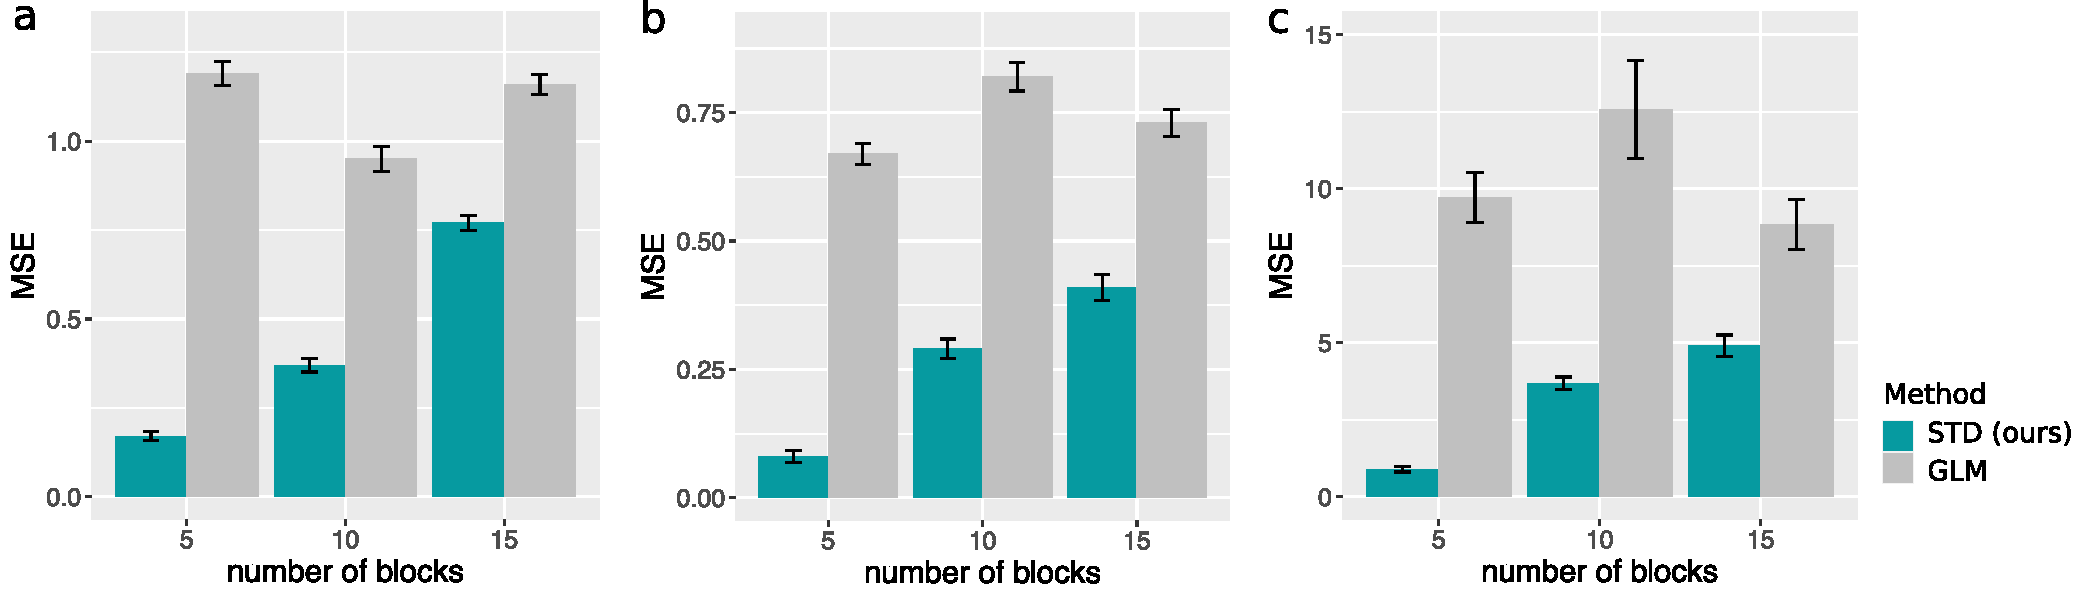
\includegraphics[width=16cm]{compare_GLM.pdf}
\caption{Performance comparison under stochastic block models. The three panels plot the MSE when the response tensors are generated from (a) Gaussian (b) Poisson and (c) Bernoulli models. The $x$-axis represents the number of blocks in the networks. }\label{fig:glm}
\end{figure}


Figure~\ref{fig:glm} compares the MSE of our method with a multiple-response GLM approach. The multiple-response GLM is to regress the dyadic edges, one at a time, on the features, and this model is repeatedly fitted for each edge. As we find in Figure~\ref{fig:glm}, our tensor regression method achieves significant error reduction in all three data types considered. The outperformance is substantial in the presence of large communities; even in the less structured case ($\sim 20/15=1.33$ nodes per block), our method still outer-performs GLM. The possible reason is that the multiple-response GLM approach does not account for the correlation among the edges, and suffers from overfitting. In contrast, the low-rankness in our modeling incorporates the shared information across entries. By selecting the rank in a data-driven way, our method achieves accurate estimation in a wide range of settings. 


\section{Additional results on data application}\label{sec:adata}
\subsection{Rank selection for Nations data}
Table~\ref{tab:rank_select} summarizes the BIC results in the grid search $\mr\in \{3,4,5\}^3$. We set $r_1=r_2$ due to the symmetry in the dataset. Table~\ref{tab:rank_select} shows that $(r_1,r_2)=(4,4)$ consistently provides the minimal BIC under a range of $r_3$. Because multiple values of $r_3$ give similar BIC, we choose $r_3$ based on the interpretability of the results. Tables~\ref{tab:s1_3}-\ref{tab:s1_5} compare the clustering results for $r_3=3,4,5$. For ease of visualisation, we list only the subset of relations for which the three configurations yield incoherent clustering. We find that the clustering with $r_3 = 4$ (Table~\ref{tab:s1_4}) provides the cleanest results. Table~\ref{tab:s1_3} with $r_3 = 3$ mixes the categories Economics with Organization and Military. Table~\ref{tab:s1_5} with $r_3 = 5$ mixes Economics with Organization, while splitting Military and Territory into different clusters. Therefore, we choose the rank $\mr=(4,4,4)$ in the main paper. The running time for the rank selection via grid search is 95 secs in total, on an iMac macOS High Sierra 10.13.6 with Intel Core i5 3.8 GHz CPU and 8 GB RAM. This indicates the BIC is feasible in the considered setting. 


     \begingroup
     \setlength{\tabcolsep}{4.5pt} % Default value: 6pt
    \renewcommand{\arraystretch}{1} % Default value: 1
     \begin{table}[htb]
         \centering
         \begin{tabular}{c||ccc|ccc|ccc}
         $r_3$ & \multicolumn{3}{c|}{ $r_3 = 3$} & \multicolumn{3}{c|}{ $r_3 = 4$} & \multicolumn{3}{c}{ $r_3 = 5$}\\
         \hline
             $(r_1,r_2)$ & $(3,3)$ &  $(4,4)$ &  $(5,5)$ & $(3,3)$ &  $(4,4)$ &  $(5,5)$ &  $(3,3)$ &  $(4,4)$ &  $(5,5)$ \\
             \hline\hline
              % $\ell_{\tY}$& -4733& {\bf -4560}& -4715 & -4919& {\bf -4609} & -4703 & -7347 & {\bf -4700} &-7259 \\
              BIC& 11364 & {\bf 11194} & 11701 & 12275 & {\bf 11897} & 12365 & 17652 & {\bf 12666} & 18146\\
         \end{tabular}
         \caption{BIC results for {\it Nations} data under different tensor rank. Bold number indicates the minimal BIC with a certain $r_3$. }
         \label{tab:rank_select}
     \end{table}
     \endgroup
     
     
      
     \begin{table}[h!]
    \resizebox{1\textwidth}{!}{%
    \begin{tabular}{c|l}
     Cluster& \multicolumn{1}{c}{Relations}\\
    \hline
    \multirow{2}{*}{ I}  & \textcolor{YellowOrange}{exportbooks}, \textcolor{YellowOrange}{relexportbooks}, \textcolor{OliveGreen}{protests}, \textcolor{YellowOrange}{tourism}, \textcolor{YellowOrange}{reltourism}, \textcolor{Blue}{relintergovorgs}\\
    & \textcolor{Blue}{relngo}, \textcolor{Blue}{intergovorgs3}, \textcolor{Blue}{ngoorgs3}, \textcolor{OliveGreen}{militaryalliance},\textcolor{OliveGreen}{commonbloc1} \\
    \hline
    \multirow{2}{*}{ II}  & \textcolor{OliveGreen}{militaryactions}, \textcolor{OliveGreen}{severdiplomatic},\textcolor{OliveGreen}{expeldiplomats}, \textcolor{OliveGreen}{commonbloc0},
    \textcolor{BrickRed}{aidenemy} \\ & \textcolor{BrickRed}{attackembassy},  \textcolor{BrickRed}{lostterritory},    \textcolor{OliveGreen}{blockpositionindex} \\
    \hline
    \multirow{2}{*}{III} & \textcolor{YellowOrange}{tourism3}, \textcolor{YellowOrange}{exports}, \textcolor{YellowOrange}{relexports}, \textcolor{YellowOrange}{exports3}, \textcolor{Blue}{intergovorgs}, \\ & 
    \textcolor{Blue}{ngo} ,\textcolor{OliveGreen}{ embassy}, \textcolor{OliveGreen}{reldiplomacy}, \textcolor{OliveGreen}{commonbloc2} \\
    \hline
     \multicolumn{2}{l}{ \footnotesize \fcolorbox{black}{YellowOrange}{\hspace{2mm}} 
     \raisebox{-1mm}{Economics} \quad   \fcolorbox{black}{OliveGreen}{\hspace{2mm}}  \raisebox{-1mm}{ Military}\quad \fcolorbox{black}{Blue}{\hspace{2mm}} \raisebox{-1mm}{Organization} \quad  \fcolorbox{black}{BrickRed}{\hspace{2mm}} \raisebox{-1mm}{Territory}}
    \end{tabular}
    }
    \caption{$K$-mean relations clustering with $r_3 = 3$. For visualization purpose, only a subset of relations are presented. See texts for details.}\label{tab:s1_3}
    \end{table}
    
    \begin{table}[H]
    \resizebox{1\textwidth}{!}{%
    \begin{tabular}{c|l}
     Cluster& \multicolumn{1}{c}{Relations}\\
    \hline
    \multirow{1}{*}{ I} &\textcolor{BrickRed}{aidenemy}, \textcolor{BrickRed}{attackembassy}, \textcolor{BrickRed}{lostterritory}\\
    \hline
    \multirow{2}{*}{ II}  &\textcolor{OliveGreen}{militaryactions}, \textcolor{OliveGreen}{severdiplomatic}, \textcolor{OliveGreen}{expeldiplomats}, \textcolor{OliveGreen}{protests}, \\
    & \textcolor{OliveGreen}{commonbloc0}, \textcolor{OliveGreen}{blockpositionindex}, \textcolor{OliveGreen}{commonbloc1}\\
    \hline
    \multirow{1}{*}{III} & \textcolor{Blue}{relintergovorgs}, \textcolor{Blue}{relngo}, \textcolor{Blue}{intergovorgs3}, \textcolor{Blue}{ngoorgs3}, \textcolor{OliveGreen}{militaryalliance}, \textcolor{OliveGreen}{commonbloc2}\\
    \hline
    \multirow{2}{*}{IV} &\textcolor{YellowOrange}{exportbooks}, \textcolor{YellowOrange}{relexportbooks}, \textcolor{YellowOrange}{tourism}, \textcolor{YellowOrange}{reltourism}, \textcolor{YellowOrange}{tourism3} \\
    &\textcolor{YellowOrange}{exports}, \textcolor{YellowOrange}{relexports}, \textcolor{YellowOrange}{exports3}, \textcolor{Blue}{intergovorgs}, \textcolor{Blue}{ngo}, \textcolor{OliveGreen}{embassy}, \textcolor{OliveGreen}{reldiplomacy}\\
    \hline
    \multicolumn{2}{l}{ \footnotesize   \fcolorbox{black}{YellowOrange}{\hspace{2mm}} \raisebox{-1mm}{Economics} \quad 
 \fcolorbox{black}{OliveGreen}{\hspace{2mm}}    \raisebox{-1mm}{Military}\quad \fcolorbox{black}{Blue}{\hspace{2mm}}  \raisebox{-1mm}{Organization} \quad  \fcolorbox{black}{BrickRed}{\hspace{2mm}}  \raisebox{-1mm}{Territory}}
    \end{tabular}
    }
    \caption{$K$-mean relations clustering with $r_3 = 4$. For visualization purpose, only a subset of relations are presented. See texts for details.}\label{tab:s1_4}
    \end{table}
    
    \begin{table}[H]
    \resizebox{\textwidth}{!}{%
    \begin{tabular}{c|l}
     Cluster& \multicolumn{1}{c}{Relations}\\
    \hline
    \multirow{2}{*}{ I} &\textcolor{YellowOrange}{exportbooks}, \textcolor{YellowOrange}{relexportbooks}, \textcolor{YellowOrange}{tourism}, \textcolor{YellowOrange}{reltourism}, \textcolor{YellowOrange}{tourism3}, \textcolor{YellowOrange}{exports}, \textcolor{YellowOrange}{relexports}, \textcolor{YellowOrange}{exports3}\\
    &\textcolor{Blue}{intergovorgs}, \textcolor{Blue}{relintergovorgs}, \textcolor{Blue}{ngo}, \textcolor{Blue}{relngo}, \textcolor{Blue}{intergovorgs3}, \textcolor{Blue}{ngoorgs3}, \textcolor{OliveGreen}{embassy}, \textcolor{OliveGreen}{reldiplomacy}\\
    \hline
    \multirow{1}{*}{ II}  &\textcolor{BrickRed}{attackembassy}\\
    \hline
    \multirow{1}{*}{III} & \textcolor{OliveGreen}{commonbloc0}, \textcolor{OliveGreen}{blockpositionindex}\\
    \hline
    \multirow{1}{*}{IV} & \textcolor{OliveGreen}{militaryalliance}, \textcolor{OliveGreen}{commonbloc2}\\
    \hline
    \multirow{2}{*}{V} & \textcolor{OliveGreen}{militaryactions}, \textcolor{OliveGreen}{severdiplomatic}, \textcolor{OliveGreen}{expeldiplomats}, \textcolor{BrickRed}{aidenemy}, \textcolor{BrickRed}{lostterritory},\\ & \textcolor{OliveGreen}{protests}, \textcolor{OliveGreen}{commonbloc1}\\
    \hline
    \multicolumn{2}{l}{ \footnotesize \fcolorbox{black}{YellowOrange}{\hspace{2mm}} \raisebox{-1mm}{Economics} \quad   \fcolorbox{black}{OliveGreen}{\hspace{2mm}}   \raisebox{-1mm}{Military}\quad \fcolorbox{black}{Blue}{\hspace{2mm}} \raisebox{-1mm}{Organization} \quad 
    \fcolorbox{black}{BrickRed}{\hspace{2mm}} \raisebox{-1mm}{Territory}}
    \end{tabular}
    }
    \caption{$K$-mean relations clustering with $r_3 = 5$. For visualization purpose, only a subset of relations are presented. See texts for details.}\label{tab:s1_5}
    \end{table}
    


\subsection{Comparison with unsupervised decomposition}\label{sec:compare1}

We compare the supervised vs.\ unsupervised decomposition in the {\it Nations} data analysis. Table~\ref{tab:unsup} shows the clustering results based on classical unsupervised Tucker decomposition without the feature matrices. Table~\ref{tab:s1} shows the clustering results based on supervised tensor decomposition ({\bf STD}). Compared with supervised decomposition, the unsupervised clustering loses some interpretation. Similar relations {\it exports} and {\it relexports}, {\it ngo} and {\it relngo} are separated into different clusters. 


\begin{table}[!h]
    \resizebox{\textwidth}{!}{%
    \begin{tabular}{c|l}
     Cluster& \multicolumn{1}{c}{Relations}\\
    \hline
    \multirow{2}{*}{ I}  &\textcolor{YellowOrange}{economicaid}, \textcolor{YellowOrange}{releconomicaid}, \textcolor{YellowOrange}{exportbooks}, \textcolor{YellowOrange}{relexportbooks}, \textcolor{OliveGreen}{weightedunvote}, \textcolor{OliveGreen}{unweightedunvote}, \\
    &\textcolor{YellowOrange}{tourism}, \textcolor{YellowOrange}{reltourism}, \textcolor{YellowOrange}{tourism3}, \textcolor{YellowOrange}{exports}, \textcolor{Blue}{intergovorgs}, \textcolor{Blue}{ngo}, \textcolor{OliveGreen}{militaryalliance}\\
    \hline
    \multirow{2}{*}{ II}  & \textcolor{OliveGreen}{warning}, \textcolor{OliveGreen}{violentactions}, \textcolor{OliveGreen}{militaryactions}, \textcolor{OliveGreen}{duration}, \textcolor{OliveGreen}{severdiplomatic}, \textcolor{OliveGreen}{expeldiplomats}, \textcolor{YellowOrange}{boycottembargo}, \textcolor{BrickRed}{aidenemy}, \\
    &\textcolor{OliveGreen}{negativecomm}, \textcolor{Blue}{accusation}, \textcolor{OliveGreen}{protests}, \textcolor{OliveGreen}{unoffialacts}, \textcolor{BrickRed}{attackembassy}, \textcolor{Blue}{relemigrants}, \textcolor{OliveGreen}{timesincewar}, \textcolor{BrickRed}{lostterritory}, \textcolor{OliveGreen}{dependent}\\
    \hline
    III & \textcolor{OliveGreen}{timesinceally}, \textcolor{OliveGreen}{independence}, \textcolor{OliveGreen}{commonbloc0}, \textcolor{OliveGreen}{blockpositionindex}\\
    \hline
    \multirow{3}{*}{IV}  &\textcolor{YellowOrange}{treaties}, \textcolor{YellowOrange}{reltreaties}, \textcolor{YellowOrange}{officialvisits}, \textcolor{YellowOrange}{conferences}, \textcolor{YellowOrange}{booktranslations}, \textcolor{YellowOrange}{relbooktranslations}\\
    &\textcolor{OliveGreen}{negativebehavior}, \textcolor{Blue}{nonviolentbehavior}, \textcolor{Blue}{emigrants}, \textcolor{Blue}{emigrants3}, \textcolor{Blue}{students}, \textcolor{Blue}{relstudents}, \textcolor{YellowOrange}{relexports}, \textcolor{YellowOrange}{exports3}\\
    & \textcolor{Blue}{relintergovorgs}, \textcolor{Blue}{relngo}, \textcolor{Blue}{intergovorgs3}, \textcolor{Blue}{ngoorgs3}, \textcolor{OliveGreen}{embassy}, \textcolor{OliveGreen}{reldiplomacy}, \textcolor{OliveGreen}{commonbloc1}, \textcolor{OliveGreen}{commonbloc2}\\
    \hline
    \multicolumn{2}{l}{ \footnotesize \fcolorbox{black}{YellowOrange}{\hspace{2mm}} \raisebox{-1mm}{Economics} \quad   \fcolorbox{black}{OliveGreen}{\hspace{2mm}}   \raisebox{-1mm}{Military}\quad \fcolorbox{black}{Blue}{\hspace{2mm}} \raisebox{-1mm}{Organization} \quad 
    \fcolorbox{black}{BrickRed}{\hspace{2mm}} \raisebox{-1mm}{Territory}}
    \end{tabular}
    }
    \caption{Clustering of relations based on unsupervised tensor decomposition. }\label{tab:unsup}
    \end{table}


\begin{table}[!h]
\resizebox{\textwidth}{!}{%
\begin{tabular}{c|l}
 Category & \multicolumn{1}{c}{Relations}\\
\hline
\multirow{2}{*}{ I}   & \textcolor{OliveGreen}{warning}, \textcolor{OliveGreen}{violentactions}, \textcolor{OliveGreen}{militaryactions}, \textcolor{OliveGreen}{duration}, \textcolor{OliveGreen}{negativebehavior}, \textcolor{OliveGreen}{protests}, \textcolor{OliveGreen}{severdiplomatic} \\
&\textcolor{OliveGreen}{timesincewar}, \textcolor{OliveGreen}{commonbloc0}, \textcolor{OliveGreen}{commonbloc1}, \textcolor{OliveGreen}{blockpositionindex},  \textcolor{OliveGreen}{expeldiplomats}\\   
\hline
\multirow{2}{*}{II}& \textcolor{Blue}{emigrants}, \textcolor{Blue}{emigrants3}, \textcolor{Blue}{relemigrants}, \textcolor{Blue}{accusation}, \textcolor{Blue}{nonviolentbehavior}, \textcolor{Blue}{ngoorgs3}, \textcolor{OliveGreen}{commonbloc2}, \textcolor{Blue}{intergovorgs3}\\      
&\textcolor{YellowOrange}{releconomicaid}, \textcolor{Blue}{relintergovorgs}, \textcolor{Blue}{relngo},  \textcolor{Blue}{students}, \textcolor{Blue}{relstudents}, \textcolor{YellowOrange}{economicaid}, \textcolor{OliveGreen}{negativecomm}, \textcolor{OliveGreen}{militaryalliance} \\
\hline
\multirow{3}{*}{ III} & \textcolor{YellowOrange}{treaties}, \textcolor{YellowOrange}{reltreaties}, \textcolor{YellowOrange}{officialvisits}, \textcolor{YellowOrange}{exportbooks}, \textcolor{YellowOrange}{relexportbooks}, \textcolor{YellowOrange}{booktranslations}, \textcolor{YellowOrange}{relbooktranslations}\\
&\textcolor{YellowOrange}{boycottembargo}, \textcolor{OliveGreen}{weightedunvote}, \textcolor{OliveGreen}{unweightedunvote}, \textcolor{YellowOrange}{reltourism}, \textcolor{YellowOrange}{tourism}, \textcolor{YellowOrange}{tourism3}, \textcolor{YellowOrange}{exports}, \textcolor{YellowOrange}{exports3}  \\
&\textcolor{YellowOrange}{relexports}, \textcolor{Blue}{intergovorgs}, \textcolor{Blue}{ngo}, \textcolor{OliveGreen}{embassy}, \textcolor{OliveGreen}{reldiplomacy}, \textcolor{OliveGreen}{timesinceally}, \textcolor{OliveGreen}{independence}, \textcolor{YellowOrange}{conferences}, \textcolor{OliveGreen}{dependent}\\
\hline
IV &\textcolor{BrickRed}{aidenemy}, \textcolor{BrickRed}{lostterritory}, \textcolor{OliveGreen}{unoffialacts}, \textcolor{BrickRed}{attackembassy}\\
\hline
\multicolumn{2}{l}{ \footnotesize \fcolorbox{black}{YellowOrange}{\hspace{2mm}} \raisebox{-1mm}{Economics} \quad   \fcolorbox{black}{OliveGreen}{\hspace{2mm}}   \raisebox{-1mm}{Military}\quad \fcolorbox{black}{Blue}{\hspace{2mm}} \raisebox{-1mm}{Organization} \quad 
    \fcolorbox{black}{BrickRed}{\hspace{2mm}} \raisebox{-1mm}{Territory}}
\end{tabular}
}
\caption{Clustering of relations based on supervised tensor decomposition. }\label{tab:s1}
\end{table}

\subsection{How different are supervised vs.\ unsupervised factors in general?}\label{sec:compare2}
It is helpful to realize that the unsupervised and methods address different aspects of the problem. The unsupervised decomposition identifies factors that explain most variation in the tensor, whereas the supervised decomposition identifies factors that are most attributable to side features. 

We provide a simple example here for illustration.
\begin{example}
Consider the following data tensor $\tY$ and one-sided feature matrix $\mX$, 
\begin{align}
    \tY = \me_1\otimes \me_1 \otimes \me_1+10\me_2\otimes \me_2 \otimes \me_2, \quad \mX=\me_1,
\end{align}
where $\me_i=(0,\ldots,0, 1,0,\ldots,0)^T$ is the $i$th canonical basis vector in $\mathbb{R}^d$ for $i=1,2$. 
Now, consider the unsupervised vs.\ supervised decomposition of $\tY$ with rank $\mr = (1,1,1)$. 
Then, the top supervised and unsupervised factors are perpendicular to each other, 
\[
\mM_{\text{sup},k} \perp \mM_{\text{unsup},k}, \quad \text{for all } k=1,2,3,
\]
where $\mM_{\text{sup},k}$, $\mM_{\text{unsup},k}$ denote the mode-$k$ factors from supervised and unsupervised decompositions, respectively. 
\end{example}

\begin{rmk}
This example shows complementary information between factors from supervised vs.\ unsupervised decompositions. In general, one could construct examples such that these two methods return {\bf arbitrarily different} factors.   
\end{rmk}

\newpage
\bibliography{tensor_wang}
\bibliographystyle{apalike}


\end{document}
